\section{实验结果}\label{sec:results}

\subsection{分布内检测}\label{sec:main-results}

表~\ref{tab:main} 给出两个数据集上的主结果。

\begin{table}[t]
\centering\footnotesize
\setlength{\tabcolsep}{3.2pt}
\caption{测试集结果（\%）。可训练方法为多个随机种子的均值，下标为标准差（LoRA-LLM 与学生模型为 3 个种子，其余为 5 个）；每列最优的可训练方法加粗。$^\dagger$ 使用 ARG 数据自带的 GPT-3.5 输出，其余 LLM 输出均来自 Qwen2.5-7B。}\label{tab:main}
\begin{tabular}{lcccccccc}
\toprule
\multirow{2}{*}{方法} & \multicolumn{4}{c}{Weibo21（中文）} & \multicolumn{4}{c}{GossipCop（英文）} \\
\cmidrule(lr){2-5}\cmidrule(lr){6-9}
 & macF1 & Acc & F1$_{\text{真}}$ & F1$_{\text{假}}$ & macF1 & Acc & F1$_{\text{真}}$ & F1$_{\text{假}}$ \\
\midrule
\multicolumn{9}{l}{\emph{仅 LLM，不训练}} \\
GPT-3.5，常识视角$^\dagger$ & 69.64 & 70.58 & 74.98 & 64.30 & 71.04 & 84.26 & 90.61 & 51.47 \\
Qwen2.5-7B，零样本 & 73.86 & 74.01 & 75.87 & 71.85 & 60.72 & 79.33 & 87.76 & 33.67 \\
Qwen2.5-7B，零样本 CoT & 73.22 & 73.35 & 75.05 & 71.40 & 62.50 & 72.42 & 81.78 & 43.21 \\
\midrule
\multicolumn{9}{l}{\emph{仅 SLM}} \\
BERT & 76.46\pmstd{0.35} & 76.56\pmstd{0.36} & 77.83\pmstd{0.84} & 75.08\pmstd{0.85} & 76.66\pmstd{1.34} & 85.74\pmstd{1.04} & 91.22\pmstd{0.69} & 62.10\pmstd{2.02} \\
\midrule
\multicolumn{9}{l}{\emph{微调 LLM}} \\
LoRA-LLM & \textbf{79.74}\pmstd{1.36} & \textbf{79.99}\pmstd{1.24} & \textbf{81.96}\pmstd{0.73} & \textbf{77.52}\pmstd{2.02} & 77.04\pmstd{0.56} & 87.04\pmstd{0.44} & 92.19\pmstd{0.30} & 61.88\pmstd{0.94} \\
\midrule
\multicolumn{9}{l}{\emph{LLM + SLM}} \\
BERT+ZS & 78.00\pmstd{0.43} & 78.08\pmstd{0.43} & 79.33\pmstd{0.57} & 76.67\pmstd{0.62} & 77.73\pmstd{0.47} & \textbf{87.31}\pmstd{0.29} & \textbf{92.34}\pmstd{0.19} & 63.12\pmstd{0.85} \\
ARG（GPT-3.5 理由）$^\dagger$ & 76.82\pmstd{1.06} & 76.99\pmstd{1.09} & 78.76\pmstd{1.23} & 74.87\pmstd{1.03} & 77.09\pmstd{1.10} & 87.07\pmstd{0.65} & 92.21\pmstd{0.41} & 61.97\pmstd{1.91} \\
ARG & 77.41\pmstd{0.97} & 77.58\pmstd{1.04} & 79.34\pmstd{1.34} & 75.47\pmstd{0.68} & 77.17\pmstd{1.04} & 86.52\pmstd{1.15} & 91.77\pmstd{0.79} & 62.56\pmstd{1.33} \\
FactGuard & 76.38\pmstd{0.80} & 76.49\pmstd{0.88} & 77.93\pmstd{1.27} & 74.84\pmstd{0.50} & 77.24\pmstd{1.01} & 86.31\pmstd{1.16} & 91.60\pmstd{0.83} & 62.87\pmstd{1.32} \\
\method{} & 77.41\pmstd{0.49} & 77.57\pmstd{0.51} & 79.31\pmstd{0.66} & 75.50\pmstd{0.48} & \textbf{78.15}\pmstd{1.06} & 86.84\pmstd{0.86} & 91.92\pmstd{0.58} & \textbf{64.38}\pmstd{1.65} \\
\midrule
\multicolumn{9}{l}{\emph{学生模型（推理时不调用 LLM）}} \\
ARG-D & 76.41\pmstd{0.50} & 76.54\pmstd{0.41} & 78.11\pmstd{0.23} & 74.71\pmstd{1.17} & -- & -- & -- & -- \\
FactGuard-D & 75.98\pmstd{0.57} & 76.10\pmstd{0.56} & 77.65\pmstd{0.57} & 74.30\pmstd{0.70} & -- & -- & -- & -- \\
\student{} & 75.98\pmstd{0.74} & 76.11\pmstd{0.76} & 77.75\pmstd{0.89} & 74.22\pmstd{0.68} & -- & -- & -- & -- \\
\bottomrule
\end{tabular}

\end{table}

\paragraph{\method{} 与已有的 LLM+SLM 方法持平，没有稳定的优势}
在 Weibo21 上 \method{} 的 macro-F1 为 \ptwo{CN/main/clara/macf1}，与 ARG（\ptwo{CN/main/arg/macf1}）几乎相同，高于 FactGuard（\ptwo{CN/main/factguard/macf1}）与 BERT（\ptwo{CN/main/bert/macf1}）约 1 个点。在 GossipCop 上 \method{} 为 \ptwo{EN/main/clara/macf1}，在 SLM 类方法中最高，比 ARG 高 \ptwo{EN/significance/arg/diff_mean} 个点。但配对 bootstrap 检验（附录表~\ref{tab:sig}）显示，除 Weibo21 上对 FactGuard 的差异（$p=\fthree{CN/significance/factguard/bootstrap/p}$）外，\method{} 与其他 SLM 类方法的差异都不显著；对 BERT 的提升在两个数据集上处于显著性边缘（$p=\fthree{CN/significance/bert/bootstrap/p}$ 与 $\fthree{EN/significance/bert/bootstrap/p}$）。分布内精度不是 \method{} 的优势所在。

\paragraph{最简单的融合方式同样有效}
BERT+ZS 只在 BERT 的输出上加了一项 LLM 零样本评分，在 Weibo21 上达到 \ptwo{CN/main/bert_zs/macf1}，是 SLM 类方法中最高的；在 GossipCop 上为 \ptwo{EN/main/bert_zs/macf1}，与 ARG、FactGuard 相当。也就是说，在分布内精度这一指标上，让 SLM 阅读 LLM 的理由文本并没有比直接使用一个 LLM 置信度分数带来更多收益。已有的 LLM+SLM 工作没有报告过这一对照。

\paragraph{直接微调 LLM 更强}
LoRA-LLM 在 Weibo21 上的 macro-F1 为 \ptwo{CN/main/lora/macf1}，在 GossipCop 上为 \ptwo{EN/main/lora/macf1}。它只需要一次前向、不需要生成任何文本，代价是训练与推理都要运行 7B 模型（\ref{sec:exp-cost} 节）。把 LLM 冻结、只训练小模型的协同范式，在本文的设置下没有达到直接微调同一个 LLM 的精度。

\paragraph{与已发表数值的关系}
ARG 论文在同样的数据上报告的 macro-F1 为 78.4（Weibo21）与 79.0（GossipCop），FactGuard 论文报告的是 80.1 与 80.5，TED 为 79.5 与 80.3。本文复现的数值更低，原因有三：其一，这些数值来自单次运行；其二，本文把理由换成了 7B 开源模型的输出；其三，实现上可能存在小的系统差异。为了量化第三点，我们在本机运行了 ARG 的官方代码（仅做库版本兼容性修改，使用其发布的配置与 GPT-3.5 理由）：官方种子得到 78.0，另一个种子得到 77.5；本文的实现在相同的输入与学习率下，5 个种子的均值为 \ptwo{CN/grid/arg_gpt@lr2e-05/test/mean}，每步重算冻结层时 3 个种子的均值为 \ptwo{CN/live/arg_gpt@lr2e-05/live/mean}（附录~\ref{app:live}）。与官方代码相差约 0.5--1 个点，与种子间的波动同一量级，但不能排除存在小的系统差。由于所有方法共用同一套实现与协议，方法之间的比较不受影响。值得注意的是，官方代码的两次运行都没有达到论文报告的 78.4，在本文的多种子设置下，这些方法之间约 1 个点的已发表差距处于随机波动范围之内。

\subsection{当 LLM 的分析不可用时}\label{sec:exp-noise}

表~\ref{tab:noise} 与图~\ref{fig:noise} 给出把 LLM 分析替换为其他新闻的分析后各方法的表现。

\begin{table}[t]
\centering\footnotesize
\setlength{\tabcolsep}{3.4pt}
\caption{LLM 分析被替换时的 macro-F1（\%，多种子均值）。“整条替换”列为被替换的测试样本比例，“单元替换”列为每个声明或理由句被替换的概率。BERT 不使用 LLM，不受影响。BERT+ZS 只使用零样本评分，单元替换不改变它的输入。}\label{tab:noise}
\begin{tabular}{lcccccccccc}
\toprule
 & \multicolumn{5}{c}{Weibo21（中文）} & \multicolumn{5}{c}{GossipCop（英文）} \\
\cmidrule(lr){2-6}\cmidrule(lr){7-11}
 & & \multicolumn{2}{c}{整条替换} & \multicolumn{2}{c}{单元替换} & & \multicolumn{2}{c}{整条替换} & \multicolumn{2}{c}{单元替换} \\
\cmidrule(lr){3-4}\cmidrule(lr){5-6}\cmidrule(lr){8-9}\cmidrule(lr){10-11}
方法 & 原始 & 40\% & 100\% & 50\% & 100\% & 原始 & 40\% & 100\% & 50\% & 100\% \\
\midrule
BERT（不使用 LLM） & 76.46 & $=$ & $=$ & $=$ & $=$ & 76.66 & $=$ & $=$ & $=$ & $=$ \\
BERT+ZS & 78.00 & 76.49 & 74.43 & -- & -- & 77.73 & 77.15 & 76.94 & -- & -- \\
FactGuard & 76.38 & 72.46 & 67.62 & 73.94 & 69.21 & 77.24 & 71.83 & 64.63 & 73.64 & 66.45 \\
ARG & 77.41 & 76.36 & 75.74 & 76.77 & 76.00 & 77.17 & 76.27 & 75.89 & 76.24 & 76.06 \\
ARG + 错配负例 & 77.03 & 76.70 & 76.22 & 76.69 & 76.34 & 76.93 & 76.69 & 76.41 & 76.68 & 76.05 \\
\method{} & 77.41 & 76.65 & 75.53 & 77.46 & 77.55 & 78.15 & 76.34 & 75.83 & 77.00 & 76.23 \\
\bottomrule
\end{tabular}

\end{table}

\begin{figure}[t]
\centering
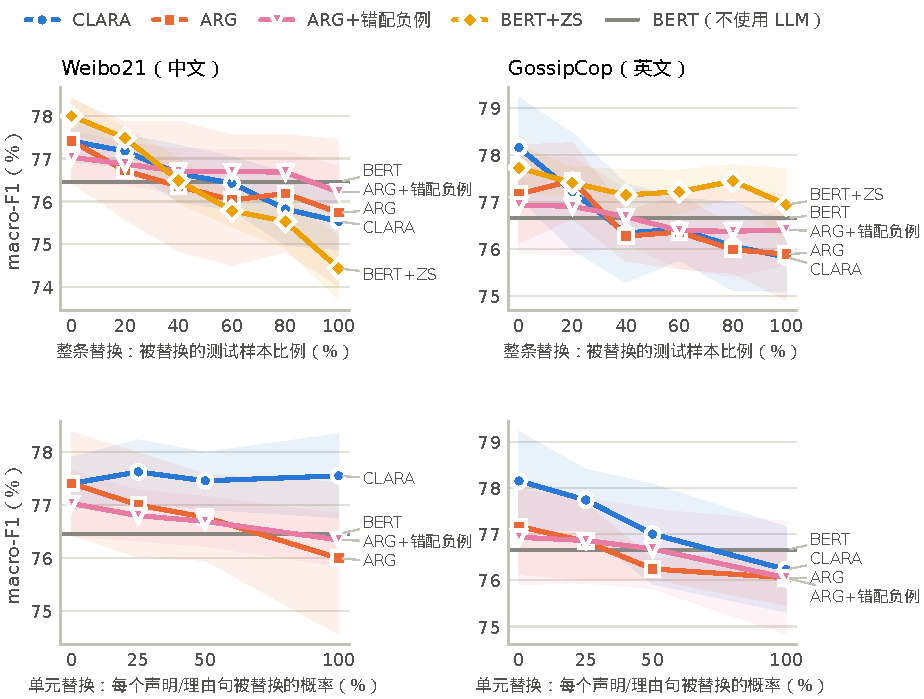
\includegraphics[width=\linewidth]{figures/noise.pdf}
\caption{LLM 分析被替换时的 macro-F1。上：整条替换；下：单元替换。阴影为种子间标准差，灰色横线为不使用 LLM 的 BERT。数值见表~\ref{tab:noise}。}\label{fig:noise}
\end{figure}

\paragraph{相关性门控能识别不属于该新闻的分析}
表~\ref{tab:gate} 显示，相关性门控 $r$ 几乎完美地区分了属于本新闻的分析单元与被替换进来的单元：整条替换时 AUC 为 \fthree{CN/gate/relevance/item/auc_r}（Weibo21）与 \fthree{EN/gate/relevance/item/auc_r}（GossipCop），单元替换时为 \fthree{CN/gate/relevance/unit/auc_r} 与 \fthree{EN/gate/relevance/unit/auc_r}。属于本新闻的单元平均 $r$ 在 0.93 以上，被替换的单元在 0.2 以下。判定门控 $g$ 则完全不具备这一能力（AUC 约 0.5）。

\begin{table}[t]
\centering\small
\caption{相关性门控对“分析单元是否属于该新闻”的区分能力（测试集，多种子均值）。}\label{tab:gate}
\begin{tabular}{lcccc}
\toprule
 & \multicolumn{2}{c}{Weibo21（中文）} & \multicolumn{2}{c}{GossipCop（英文）} \\
\cmidrule(lr){2-3}\cmidrule(lr){4-5}
 & 整条替换 & 单元替换 & 整条替换 & 单元替换 \\
\midrule
AUC：相关性门控 $r$ $\rightarrow$ 是否为本新闻的分析 & 0.996 & 0.992 & 0.994 & 0.989 \\
AUC：判定门控 $g$ $\rightarrow$ 同上 & 0.537 & 0.516 & 0.501 & 0.499 \\
本新闻的分析单元上的平均 $r$ & 0.930 & 0.958 & 0.947 & 0.957 \\
被替换的分析单元上的平均 $r$ & 0.169 & 0.098 & 0.182 & 0.132 \\
\bottomrule
\end{tabular}

\end{table}

\paragraph{去掉相关性门控后模型在替换下崩溃}
消融实验（表~\ref{tab:ablation}）中“去掉相关性门控与错配负例”的变体，在全部分析被整条替换时，Weibo21 上的 macro-F1 从 \ptwo{CN/ablation/full/noise100/mean} 降到 \ptwo{CN/ablation/no_relevance/noise100/mean}，远低于不使用 LLM 的 BERT。加入相关性门控后，\method{} 在同样条件下保持在 \ptwo{CN/noise/clara/item/100/mean}（Weibo21）与 \ptwo{EN/noise/clara/item/100/mean}（GossipCop），比 BERT 低约 1 个点。

\paragraph{单元替换是声明级结构有优势的地方}
当分析中只有一部分单元被替换时，\method{} 可以逐条丢弃无关的声明、保留其余部分。在 Weibo21 上，即使全部声明都被替换，\method{} 的 macro-F1 仍为 \ptwo{CN/noise/clara/unit/100/mean}，与未替换时（\ptwo{CN/noise/clara/unit/0/mean}）持平：此时裁决器依靠未被替换的整体判断与文本分支。ARG 在同样条件下从 \ptwo{CN/noise/arg/unit/0/mean} 降到 \ptwo{CN/noise/arg/unit/100/mean}，两者在该条件下的差异显著（配对 bootstrap，$p=\fthree{CN/noise_sig/unit100/arg/bootstrap/p}$）。GossipCop 上没有这一优势：\method{} 从 \ptwo{EN/noise/clara/unit/0/mean} 降到 \ptwo{EN/noise/clara/unit/100/mean}，降幅大于 ARG（\ptwo{EN/noise/arg/unit/0/mean} 降到 \ptwo{EN/noise/arg/unit/100/mean}），两者最终水平相当。

\paragraph{需要如实说明的两点}
第一，ARG 本身对替换就相当稳健：整条替换全部理由后，它在两个数据集上只下降 1.3--1.7 个点。它的融合权重并不能识别被替换的理由（被替换与未被替换样本上的平均权重几乎相同，区分两者的 AUC 为 \fthree{CN/gate/weights_under_noise/arg/auc} 与 \fthree{EN/gate/weights_under_noise/arg/auc}），稳健性来自新闻文本在其表示中占主导。给 ARG 加上同样的错配负例训练后，它在整条替换下略好于 \method{}。因此，“在分析不可用时保持稳健”并不是 \method{} 独有的性质；\method{} 相对 ARG 的可测优势只出现在 Weibo21 的单元替换上。第二，FactGuard 对两种替换都非常敏感（整条替换全部分析后降到 \ptwo{CN/noise/factguard/item/100/mean} 与 \ptwo{EN/noise/factguard/item/100/mean}），因为它用 LLM 抽取的 topic-content 代替新闻原文参与交叉注意力。

\subsection{判定门控学到了什么}\label{sec:exp-gate}

判定门控 $g$ 的设计意图是估计“LLM 在该实例上是否站对了边”。表~\ref{tab:gate-cells} 按 LLM 的整体判断与新闻标签把测试样本分为四组，给出各组的平均 $g_0$。

\begin{table}[t]
\centering\small
\caption{判定门控在整体实例上的取值（测试集，多种子均值）。若门控跟随“LLM 是否正确”，则第一、四行应高，第二、三行应低。}\label{tab:gate-cells}
\begin{tabular}{llcccc}
\toprule
 & & \multicolumn{2}{c}{Weibo21（中文）} & \multicolumn{2}{c}{GossipCop（英文）} \\
\cmidrule(lr){3-4}\cmidrule(lr){5-6}
LLM 的整体判断 & 新闻标签 & 占比（\%） & 平均 $g_0$ & 占比（\%） & 平均 $g_0$ \\
\midrule
判假 & 假（LLM 对） & 33.6 & 0.805 & 5.3 & 0.564 \\
判假 & 真（LLM 错） & 17.6 & 0.656 & 7.3 & 0.815 \\
判真 & 假（LLM 错） & 8.1 & 0.810 & 13.1 & 0.692 \\
判真 & 真（LLM 对） & 40.7 & 0.625 & 74.3 & 0.842 \\
\midrule
\multicolumn{2}{l}{AUC：$g_0$ $\rightarrow$ LLM 的整体判断是否正确} & \multicolumn{2}{c}{0.482} & \multicolumn{2}{c}{0.680} \\
\multicolumn{2}{l}{AUC：$g_0$ $\rightarrow$ 新闻是否为假} & \multicolumn{2}{c}{0.745} & \multicolumn{2}{c}{0.192} \\
\multicolumn{2}{l}{AUC：LLM 自身置信度 $\rightarrow$ 判断是否正确} & \multicolumn{2}{c}{0.532} & \multicolumn{2}{c}{0.510} \\
\multicolumn{2}{l}{AUC：文本分支与 LLM 是否一致 $\rightarrow$ 判断是否正确} & \multicolumn{2}{c}{0.760} & \multicolumn{2}{c}{0.858} \\
\bottomrule
\end{tabular}

\end{table}

\paragraph{判定门控跟随的是新闻标签，而不是 LLM 的正误}
在 Weibo21 上，$g_0$ 在两组假新闻上都高（约 0.81），在两组真新闻上都低（约 0.63--0.66），与 LLM 判断的方向无关：它预测“LLM 是否正确”的 AUC 为 \fthree{CN/gate/clara/overall/auc_gate/mean}，预测“新闻是否为假”的 AUC 却有 \fthree{CN/gate/clara/overall/auc_gate_for_label/mean}。在 GossipCop 上情形相反，$g_0$ 在真新闻上更高，对“LLM 是否正确”的 AUC 为 \fthree{EN/gate/clara/overall/auc_gate/mean}，但这同样可以由标签解释：该数据集上 LLM 多数时候判真，“LLM 正确”与“新闻为真”高度重合。也就是说，一个能看到新闻文本的门控学到的是“这条新闻像不像假新闻”，并据此调节 LLM 证据的权重。它起到的是让 LLM 证据的权重随文本先验变化的作用，而不是可靠性估计。

\paragraph{这一现象并非 \method{} 独有}
ARG 的理由可用性预测器对“该理由对应的 LLM 判断是否正确”的 AUC 看起来不低（表~\ref{tab:useful}），但决定融合权重的打分模块对同一目标的 AUC 只有 0.50--0.55。可用性预测器同时读取新闻与理由：新闻文本提示标签，理由文本提示 LLM 的判断，两者一比较即可得到监督目标。表中“自身预测”一列用 ARG 最终的预测概率与 LLM 判断是否一致来预测同一目标，不需要任何专门的模块，得到的 AUC 与可用性预测器相当或更高。可见可用性预测器并没有提供分类器自身判断之外的信息。

\begin{table}[t]
\centering\small
\caption{对“该理由对应的 LLM 判断是否正确”的 AUC（测试集，多种子均值）：ARG 的可用性预测器、融合权重，以及“ARG 自身的最终预测与 LLM 判断是否一致”。}\label{tab:useful}
\begin{tabular}{llcccccc}
\toprule
 & & \multicolumn{3}{c}{Weibo21（中文）} & \multicolumn{3}{c}{GossipCop（英文）} \\
\cmidrule(lr){3-5}\cmidrule(lr){6-8}
模型 & 理由 & 可用性预测 & 融合权重 & 自身预测 & 可用性预测 & 融合权重 & 自身预测 \\
\midrule
ARG & 文字描述 & 0.757 & 0.548 & 0.778 & 0.882 & 0.521 & 0.887 \\
 & 常识 & 0.762 & 0.500 & 0.796 & 0.913 & 0.523 & 0.910 \\
ARG + 错配负例 & 文字描述 & 0.754 & 0.452 & 0.774 & 0.877 & 0.666 & 0.885 \\
 & 常识 & 0.773 & 0.550 & 0.790 & 0.902 & 0.575 & 0.908 \\
\bottomrule
\end{tabular}

\end{table}

\paragraph{LLM 自身的置信度也不提供这一信息}
LLM 评分偏离 0.5 的程度对其判断是否正确的 AUC 只有 \fthree{CN/gate/clara/overall/auc_llm_conf/mean} 与 \fthree{EN/gate/clara/overall/auc_llm_conf/mean}。真正有信息量的是“文本分支是否同意 LLM”（AUC \fthree{CN/gate/clara/overall/auc_text_agreement/mean} 与 \fthree{EN/gate/clara/overall/auc_text_agreement/mean}），而这一信息在加性融合中已经被隐式使用。综合来看，在闭卷条件下我们没有找到能够估计“LLM 的判断是否可靠”且不退化为预测标签的信号；本文最初设想的“声明级可靠性门控”在这一含义上没有成立，成立的是相关性门控所回答的那个更窄的问题。

\paragraph{实例概率的分布}
两个数据集上承担判定的实例不同。在 Weibo21 的假新闻中，至少有一条声明 $p_k>0.5$ 的占 \pone{CN/gate/clara/flag/fake_any_claim/mean}\%，只有整体实例 $p_0>0.5$ 的占 \pone{CN/gate/clara/flag/fake_overall_only/mean}\%，可见这里新闻级的判定主要由整体实例承担。在 GossipCop 的假新闻中，至少有一条声明 $p_k>0.5$ 的占 \pone{EN/gate/clara/flag/fake_any_claim/mean}\%，而只由整体实例触发的不到 1\%：该数据集上 LLM 的整体判断区分度很低（零样本判断的 AUC 仅 \pone{EN/style_llm/zero-shot P(fake)/auc_orig}\%），裁决器转而依靠声明实例。

\subsection{风格改写}\label{sec:exp-style}

\begin{table}[t]
\centering\small
\caption{风格改写前后的 macro-F1（\%）。只统计成功改写的样本，“原文”为同一批样本改写前的结果。分隔线以下两行是只读取 LLM 输出文本、不读新闻原文的 BERT。}\label{tab:style}
\begin{tabular}{lcccccc}
\toprule
 & \multicolumn{3}{c}{Weibo21（中文）} & \multicolumn{3}{c}{GossipCop（英文）} \\
\cmidrule(lr){2-4}\cmidrule(lr){5-7}
方法 & 原文 & 改写后 & $\Delta$ & 原文 & 改写后 & $\Delta$ \\
\midrule
BERT & 76.09\pmstd{0.38} & 50.82\pmstd{2.03} & -25.27 & 76.66\pmstd{1.34} & 64.76\pmstd{1.72} & -11.89 \\
LoRA-LLM & 79.90\pmstd{1.09} & \textbf{60.56}\pmstd{1.07} & -19.34 & 77.04\pmstd{0.56} & \textbf{72.64}\pmstd{0.65} & -4.40 \\
BERT+ZS & 77.70\pmstd{0.56} & 52.62\pmstd{1.43} & -25.08 & 77.73\pmstd{0.47} & 66.80\pmstd{1.71} & -10.92 \\
ARG & 77.10\pmstd{0.90} & 50.94\pmstd{5.14} & -26.16 & 77.17\pmstd{1.04} & 64.91\pmstd{1.26} & -12.26 \\
FactGuard & 75.90\pmstd{0.82} & 53.26\pmstd{4.18} & -22.64 & 77.24\pmstd{1.01} & 68.79\pmstd{1.97} & -8.45 \\
\method{} & 77.35\pmstd{0.46} & 53.08\pmstd{2.13} & -24.28 & 78.15\pmstd{1.06} & 68.06\pmstd{0.45} & -10.09 \\
\student{} & 75.53\pmstd{0.79} & 50.15\pmstd{1.15} & -25.37 & -- & -- & -- \\
\bottomrule
\end{tabular}

\end{table}

\paragraph{所有闭卷检测器都主要依赖文风}
把假新闻改写为通稿文风、真新闻改写为营销号文风后，Weibo21 上所有 SLM 类方法的 macro-F1 从 76--78 降到 51--53，接近随机；GossipCop 上从约 77 降到 65--69（表~\ref{tab:style}）。在 Weibo21 上各 SLM 类方法改写后的差异都在种子波动之内；在 GossipCop 上，FactGuard 与 \method{} 改写后比 BERT 高约 3--4 个点，这两种方法都使用了 LLM 对新闻内容的重新表述（topic-content 或声明），其文风与原文不同。直接微调的 LoRA-LLM 下降较少，但同样明显。

\paragraph{LLM 自身的判断同样依赖文风}
表~\ref{tab:style-llm} 不涉及任何训练，只比较 Qwen2.5-7B 对同一批样本改写前后的评分。零样本判断的 AUC 在 Weibo21 上从 \pone{CN/style_llm/zero-shot P(fake)/auc_orig} 降到 \pone{CN/style_llm/zero-shot P(fake)/auc_style}，在 GossipCop 上从 \pone{EN/style_llm/zero-shot P(fake)/auc_orig} 降到 \pone{EN/style_llm/zero-shot P(fake)/auc_style}。声明级怀疑度在改写后对真假新闻几乎没有区分度。这说明 LLM 在闭卷条件下给出的“常识分析”“声明核查”，其判别力主要来自文本的表面特征，而不是对事实的掌握。把 LLM 的分析拆得更细并不能改变这一点：声明是从改写后的文本中抽取的，其措辞与评分仍然随文风变化。

\begin{table}[t]
\centering\small
\caption{Qwen2.5-7B 的评分在风格改写前后对真假新闻的区分能力（不涉及训练）。均值差为假新闻与真新闻平均评分之差。}\label{tab:style-llm}
\begin{tabular}{lcccccccc}
\toprule
 & \multicolumn{4}{c}{Weibo21（中文）} & \multicolumn{4}{c}{GossipCop（英文）} \\
\cmidrule(lr){2-5}\cmidrule(lr){6-9}
 & \multicolumn{2}{c}{AUC（\%）} & \multicolumn{2}{c}{均值差（假$-$真）} & \multicolumn{2}{c}{AUC（\%）} & \multicolumn{2}{c}{均值差（假$-$真）} \\
LLM 评分 & 原文 & 改写 & 原文 & 改写 & 原文 & 改写 & 原文 & 改写 \\
\midrule
零样本判断 $p_{\mathrm{zs}}$ & 83.2 & 58.7 & 0.50 & 0.13 & 67.4 & 50.9 & 0.20 & 0.04 \\
整体判断的怀疑度 $v_0$ & 75.8 & 54.9 & 0.13 & 0.02 & 65.6 & 57.0 & 0.06 & 0.03 \\
声明怀疑度的最大值 & 71.0 & 50.7 & 0.11 & 0.00 & 58.5 & 56.0 & 0.03 & 0.02 \\
声明怀疑度的均值 & 72.6 & 51.2 & 0.11 & 0.01 & 56.2 & 52.7 & 0.02 & 0.01 \\
\bottomrule
\end{tabular}

\end{table}

\subsection{单句事实篡改：敏感性与定位}\label{sec:exp-loc}

\begin{table}[t]
\centering\small
\caption{对单句事实篡改的敏感性（\%）。“判假”为被判为假的比例；成对正确率为篡改后样本的预测概率高于其原文的比例，50\% 相当于随机。}\label{tab:tamper}
\begin{tabular}{lcccccc}
\toprule
 & \multicolumn{3}{c}{Weibo21（中文）} & \multicolumn{3}{c}{GossipCop（英文）} \\
\cmidrule(lr){2-4}\cmidrule(lr){5-7}
方法 & 原文判假 & 篡改后判假 & 成对正确率 & 原文判假 & 篡改后判假 & 成对正确率 \\
\midrule
BERT & 22.7 & 22.9 & 54.6 & 9.0 & 9.2 & 53.4 \\
LoRA-LLM & 15.7 & 18.2 & 68.8 & -- & -- & -- \\
BERT+ZS & 21.8 & 23.4 & 60.6 & 6.1 & 6.4 & 57.4 \\
ARG & 19.3 & 19.7 & 55.4 & 7.5 & 7.9 & 53.5 \\
FactGuard & 22.0 & 23.1 & 54.1 & 8.3 & 8.8 & 53.3 \\
\method{} & 20.0 & 21.1 & 54.8 & 8.0 & 8.6 & 53.1 \\
\bottomrule
\end{tabular}

\end{table}

\paragraph{没有方法对局部事实改动敏感}
表~\ref{tab:tamper} 显示，把真新闻中的一句话改成与原文事实不符的陈述后，各方法判其为假的比例几乎不变（例如 \method{} 在 Weibo21 上从 \pone{CN/localisation/_sensitivity/clara/flag_rate_original}\% 变为 \pone{CN/localisation/_sensitivity/clara/flag_rate_tampered}\%）；篡改后的预测概率高于原文的比例只有 53\%--55\%，略高于随机。唯一稍高的是 BERT+ZS（约 57\%--61\%），因为 LLM 的零样本评分对部分改动有反应。这与风格改写的结果一致：这些检测器学到的不是“内容是否属实”。需要强调，篡改后的句子只是与原文不符，未必在现实中为假，这项测试衡量的是模型对事实内容变化的敏感程度。

\begin{table}[t]
\centering\small
\caption{被篡改句子的定位结果（\%）。“单位”为方法给出分数的粒度；声明级分数通过声明所在的句子编号映射到句子。}\label{tab:loc}
\begin{tabular}{llcccc}
\toprule
 & & \multicolumn{2}{c}{Weibo21（中文）} & \multicolumn{2}{c}{GossipCop（英文）} \\
\cmidrule(lr){3-4}\cmidrule(lr){5-6}
方法 & 单位 & Hit@1 & MRR & Hit@1 & MRR \\
\midrule
随机猜测 & 句子 & 30.0 & -- & 19.8 & -- \\
LLM 怀疑度评分（不训练） & 声明 & 35.7 & 59.2 & 22.8 & 47.1 \\
BERT + 遮挡归因 & 句子 & 33.2\pmstd{1.2} & 58.4 & 22.2\pmstd{1.0} & 46.5 \\
LoRA-LLM + 遮挡归因 & 句子 & 38.3\pmstd{1.0} & 61.9 & 24.0\pmstd{1.9} & 48.4 \\
\method{} & 声明 & 36.2\pmstd{0.8} & 59.6 & 23.2\pmstd{0.6} & 47.0 \\
\midrule
\method{}：去掉论证文本 & 声明 & 35.4\pmstd{0.7} & 59.2 & -- & -- \\
\method{}：去掉评分 & 声明 & 35.1\pmstd{0.8} & 59.0 & -- & -- \\
\bottomrule
\end{tabular}

\end{table}

\paragraph{定位结果只略高于随机}
在定位任务上（表~\ref{tab:loc}），\method{} 的 Hit@1 在 Weibo21 上为 \pone{CN/localisation/CLARA/hit@1}\%，随机猜测为 \pone{CN/localisation/CLARA/chance}\%；在 GossipCop 上为 \pone{EN/localisation/CLARA/hit@1}\%，随机为 \pone{EN/localisation/CLARA/chance}\%。训练后的裁决器并没有比直接使用 LLM 的怀疑度评分更好，与对 BERT 做遮挡归因也相差无几。原因有两个：LLM 抽取的声明只覆盖了 \pone{CN/localisation/_claim_coverage}\%（Weibo21）与 \pone{EN/localisation/_claim_coverage}\%（GossipCop）的被篡改句子；即使覆盖到，LLM 对这条声明的怀疑度也往往不比其他声明高。“只用新闻级标签即可获得声明级定位”这一预期在闭卷条件下没有实现。

\subsection{消融实验}\label{sec:exp-ablation}

\begin{table}[t]
\centering\footnotesize
\setlength{\tabcolsep}{3.4pt}
\caption{\method{} 的消融（macro-F1，\%）。“整条替换”为全部测试样本的分析被替换，“半数单元替换”为每个单元以 0.5 的概率被替换。Weibo21 为 5 个种子，GossipCop 为 3 个种子。$^{*}$ 表示与完整模型的差异在配对 bootstrap 检验下显著（$p<0.05$）。}\label{tab:ablation}
\begin{tabular}{lcccccc}
\toprule
\multirow{2}{*}{变体} & \multicolumn{3}{c}{Weibo21（中文）} & \multicolumn{3}{c}{GossipCop（英文）} \\
\cmidrule(lr){2-4}\cmidrule(lr){5-7}
 & 原始 & 整条替换 & 单元替换 & 原始 & 整条替换 & 单元替换 \\
\midrule
\method{}（完整） & 77.41\pmstd{0.49} & 75.53\pmstd{0.66} & 77.55\pmstd{0.79} & -- & -- & -- \\
\midrule
去掉声明，仅整体实例 & 77.24\pmstd{0.53} & 74.90\pmstd{0.70} & 77.24\pmstd{0.53} & -- & -- & -- \\
去掉整体实例，仅声明 & 76.91\pmstd{0.39} & 75.48\pmstd{0.43} & 75.40\pmstd{0.31}$^{*}$ & -- & -- & -- \\
\midrule
去掉论证文本，仅评分 & 77.19\pmstd{0.36} & 75.14\pmstd{0.36} & 77.31\pmstd{0.32} & -- & -- & -- \\
去掉评分，仅论证文本 & 75.79\pmstd{0.71}$^{*}$ & 75.93\pmstd{0.61} & 75.63\pmstd{0.66}$^{*}$ & -- & -- & -- \\
论证前评分取提示内第一印象（严格单次调用） & 76.29\pmstd{0.43} & 75.26\pmstd{0.24} & 76.33\pmstd{0.52} & -- & -- & -- \\
\bottomrule
\end{tabular}

\end{table}

表~\ref{tab:ablation} 给出各组件的消融结果，详见 \ref{sec:exp-ablation-text} 节。

\subsection{未见领域}\label{sec:exp-lodo}

\begin{table}[t]
\centering\small
\caption{Weibo21 留一领域实验的 macro-F1（\%，3 个种子）。训练与验证数据不含被留出的领域。}\label{tab:lodo}
\begin{tabular}{lrrcccc}
\toprule
留出领域 & 训练数 & 测试数 & BERT & BERT+ZS & ARG & \method{} \\
\midrule
医药健康 & 4,100 & 271 & 73.82\pmstd{0.76} & \textbf{79.96}\pmstd{0.97} & 76.69\pmstd{2.41} & 75.02\pmstd{3.06} \\
政治 & 3,950 & 126 & 76.42\pmstd{3.30} & \textbf{79.59}\pmstd{0.44} & 77.75\pmstd{0.80} & 76.69\pmstd{1.22} \\
文体娱乐 & 3,444 & 134 & \textbf{73.38}\pmstd{2.86} & 71.43\pmstd{0.92} & 68.66\pmstd{2.44} & 70.64\pmstd{0.68} \\
灾难事故 & 4,135 & 185 & \textbf{79.05}\pmstd{1.60} & 78.84\pmstd{1.66} & 78.70\pmstd{1.27} & 77.78\pmstd{1.59} \\
社会生活 & 2,952 & 391 & 75.99\pmstd{1.05} & \textbf{78.74}\pmstd{0.67} & 78.04\pmstd{0.85} & 76.17\pmstd{0.46} \\
财经商业 & 3,997 & 344 & 53.62\pmstd{3.04} & \textbf{56.52}\pmstd{3.41} & 54.14\pmstd{0.53} & 56.48\pmstd{0.77} \\
\midrule
各领域平均 & & & 72.05 & \textbf{74.18}$^{*}$ & 72.33 & 72.13 \\
\bottomrule
\end{tabular}

\end{table}

\subsection{拒答}\label{sec:exp-selective}

\begin{table}[t]
\centering\small
\caption{选择性预测。AURC 越低越好；Acc@$c$ 为保留置信度最高的 $c\%$ 样本时的准确率（\%）。“选择器”为在验证集上拟合的逻辑回归。}\label{tab:selective}
\begin{tabular}{lcccccc}
\toprule
 & \multicolumn{3}{c}{Weibo21（中文）} & \multicolumn{3}{c}{GossipCop（英文）} \\
\cmidrule(lr){2-4}\cmidrule(lr){5-7}
方法 & AURC$\downarrow$ & Acc@90 & Acc@70 & AURC$\downarrow$ & Acc@90 & Acc@70 \\
\midrule
BERT & 13.75 & 79.23 & 83.25 & 6.26 & 88.60 & 91.99 \\
LoRA-LLM & 7.37 & 82.63 & 89.68 & -- & -- & -- \\
BERT+ZS & 14.44 & 80.64 & 84.14 & 5.08 & 89.88 & 92.92 \\
ARG & 12.69 & 80.40 & 85.01 & 6.77 & 89.29 & 92.83 \\
ARG + 选择器 & 12.28 & 79.87 & 83.25 & 5.97 & 89.47 & 93.35 \\
FactGuard & 17.52 & 78.93 & 82.66 & 6.50 & 89.19 & 92.26 \\
FactGuard + 选择器 & 14.57 & 78.58 & 80.85 & 6.06 & 89.29 & 92.53 \\
\method{} & 15.86 & 80.28 & 84.17 & 6.52 & 89.58 & 92.62 \\
\method{} + 选择器 & 11.11 & 80.13 & 83.51 & 5.81 & 89.68 & 93.64 \\
\bottomrule
\end{tabular}

\end{table}

\begin{figure}[t]
\centering
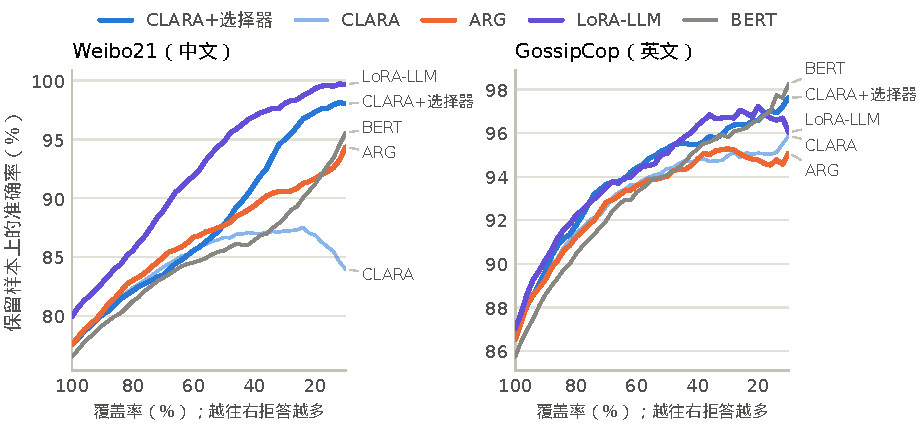
\includegraphics[width=\linewidth]{figures/selective.pdf}
\caption{保留样本上的准确率随覆盖率的变化（多种子均值）。数值见表~\ref{tab:selective}。}\label{fig:selective}
\end{figure}

\subsection{开销}\label{sec:exp-cost}

\begin{table}[t]
\centering\small
\caption{每条新闻的 LLM 开销：平均输入与输出 token 数，以及单张 RTX 3090 上用 vLLM 批量生成时每千条新闻的耗时。}\label{tab:cost}
\begin{tabular}{lccccccc}
\toprule
 & & \multicolumn{3}{c}{Weibo21（中文）} & \multicolumn{3}{c}{GossipCop（英文）} \\
\cmidrule(lr){3-5}\cmidrule(lr){6-8}
LLM 输出 & 调用数 & 输入 & 输出 & 秒/千条 & 输入 & 输出 & 秒/千条 \\
\midrule
零样本判断 & 1 & 133 & 2 & 17 & 224 & 2 & 34 \\
ARG（TD + CS 理由） & 2 & 317 & 208 & 125 & 511 & 140 & 140 \\
FactGuard（topic-content + CS 理由） & 2 & 487 & 158 & 104 & 820 & 163 & 152 \\
\method{}（结构化调用 + 零样本评分） & 2 & 791 & 283 & 182 & 984 & 438 & 319 \\
\method{}，严格单次调用 & 1 & 657 & 281 & 166 & 759 & 436 & 284 \\
\bottomrule
\end{tabular}

\end{table}

\begin{table}[t]
\centering\small
\caption{可训练参数量与单次训练耗时（单张 RTX 3090；SLM 类方法不含冻结层的一次性缓存）。}\label{tab:train-cost}
\begin{tabular}{lrrr}
\toprule
方法 & 可训练参数（M） & 训练秒数（CN） & 训练秒数（EN） \\
\midrule
BERT & 7.4 & 15 & 8 \\
BERT+ZS & 7.4 & 14 & 9 \\
ARG & 25.8 & 110 & 52 \\
FactGuard & 25.7 & 130 & 57 \\
\method{} & 20.7 & 136 & 106 \\
LoRA-LLM & 40.4 & 1940 & -- \\
\bottomrule
\end{tabular}

\end{table}
